%------------------------------------------------------------------------------
% Template file for the submission of papers to IUCr journals in LaTeX2e
% using the iucr document class
% Copyright 1999-2013 International Union of Crystallography
% Version 1.6 (28 March 2013)
%------------------------------------------------------------------------------

%xxxxxx just for testing github % 2
%xxxxxx just for testing github % 3

\documentclass[]{iucr}              % DO NOT DELETE THIS LINE
\usepackage{amssymb}
\usepackage[fleqn]{amsmath}
%\usepackage{bm}
\usepackage{graphicx}
\usepackage{tabularx}
\usepackage{booktabs}
%\usepackage{calligra}
\usepackage{array}
\DeclareMathAlphabet{\mathcalligra}{T1}{calligra}{m}{n}
\def\mathbi#1{\textbf{\em #1}}
\numberwithin{equation}{section}
%\DeclareMathSymbol{\Gamma}{\mathalpha}{letters}{"00}
%\DeclareMathSymbol{\Lambda}{\mathalpha}{letters}{"03}
%\DeclareMathSymbol{\Omega}{\mathalpha}{letters}{"0A}
%\DeclareMathAlphabet{\mathitbf}{OML}{cmm}{b}{it}
\hyphenation{Niggli}
\def\mathbi#1{\textbf{\em #1}}
%\numberwithin{equation}{section}
%\DeclareMathSymbol{\Gamma}{\mathalpha}{letters}{"00}
%\DeclareMathSymbol{\Lambda}{\mathalpha}{letters}{"03}
%\DeclareMathSymbol{\Omega}{\mathalpha}{letters}{"0A}
%\DeclareMathAlphabet{\mathitbf}{OML}{cmm}{b}{it}
\usepackage{color}
\usepackage{ulem}
\usepackage{url}
\usepackage{yfonts}
%\usepackage{xr-hyper}
%\usepackage[draft]{hyperref}
%\usepackage{bibentry}
\newcommand{\SVI}[0]{$\bf{S^{6}}$}
\newcommand{\GVI}[0]{$\bf{G^{6}}$}
\newcommand{\CIII}[0]{$\bf{C^{3}}$}
\newcommand{\DVII}[0]{$\bf{D^{7}}$}
\newcommand{\VVII}[0]{$\bf{V^{7}}$}

\newcommand{\vdotv}[2]{${{\bf #1 \cdot #2}}$}
\newcommand{\Imaginary}[0]{\mathcal{I}}
\newcommand{\Real}[0]{\mathcal{R}}
\newcommand{\Exchange}[0]{$\mathcal{X}$}

\newcommand{\nounderline}[3]{\!\!\!\!\!\!\!\!\!#1,&\!\!\!\!\!\!\!\!\!#2,&\!\!\!\!\!\!\!\!\!#3}
\newcommand{\underlineab}[3]{\!\!\!\!\!\!\!\!\!\!\!\!\!\!\!\!\!\!\!\!\!\!\!\!\Exchange{}(#1),&\!\!\!\!\!\!\!\!\!\!\!\!\!\!\!\!\!\!\!\!\!\!\!\!\Exchange{}(#2),&\!\!\!\!\!\!\!\!\!#3}
\newcommand{\underlineac}[3]{\!\!\!\!\!\!\!\!\!\!\!\!\!\!\!\!\!\!\!\!\!\!\!\!\Exchange{}(#1),&\!\!\!\!\!\!\!\!\!\!\!\!\!\!\!\!\!\!\!\!\!\!\!\!#2,&\!\!\!\!\!\!\!\!\!\Exchange{}(#3)}
\newcommand{\underlinebc}[3]{\!\!\!\!\!\!\!\!\!\!\!\!\!\!\!\!\!\!\!\!\!\!\!\!#1,&\!\!\!\!\!\!\!\!\!\Exchange{}(#2),&\!\!\!\!\!\!\!\!\!\!\!\!\!\!\!\!\!\!\!\!\!\!\!\!\Exchange{}(#3)}

\newcommand{\scalar}[1]{$#1$}

\newcommand{\scalarsub}[2]{$#1_#2$}

%-------------------------------------------------------------------------
% Information about journal to which submitted
%-------------------------------------------------------------------------
\journalcode{A}              % Indicate the journal to which submitted
%   A - Acta Crystallographica Section A
%   B - Acta Crystallographica Section B
%   C - Acta Crystallographica Section C
%   D - Acta Crystallographica Section D
%   E - Acta Crystallographica Section E
%   F - Acta Crystallographica Section F
%   J - Journal of Applied Crystallography
%   M - IUCrJ
%   S - Journal of Synchrotron Radiation
\makeatletter
\font\dummyft@=dummy \relax
\makeatother


\begin{document}                  % DO NOT DELETE THIS LINE
	
	%-------------------------------------------------------------------------
	% The introductory (header) part of the paper
	%-------------------------------------------------------------------------
	
	% The title of the paper. Use \shorttitle to indicate an abbreviated title
	% for use in running heads (you will need to uncomment it).
	
	% Authors' names and addresses. Use \cauthor for the main (contact) author.
	% Use \author for all other authors. Use \aff for authors' affiliations.
	% Use lower-case letters in square brackets to link authors to their
	% affiliations; if there is only one affiliation address, remove the [a].
	
	% Use \vita if required to give biographical details (for authors of
	% invited review papers only). Uncomment it.
	
	% lca IUCr id IUCr6401
	%\vita{Author's biography}
	
	% Keywords (required for Journal of Synchrotron Radiation only)
	% Use the \keyword macro for each word or phrase, e.g. 
	% \keyword{X-ray diffraction}\keyword{muscle}
	
	
	% PDB and NDB reference codes for structures referenced in the article and
	% deposited with the Protein Data Bank and Nucleic Acids Database (Acta
	% Crystallographica Section D). Repeat for each separate structure e.g
	% \PDBref[dethiobiotin synthetase]{1byi} \NDBref[d(G$_4$CGC$_4$)]{ad0002}
	
	%\PDBref[optional name]{refcode}
	%\NDBref[optional name]{refcode}
	
	%-------------------------------------------------------------------------
	% The introductory (header) part of the paper
	%-------------------------------------------------------------------------
	
	% The title of the paper. Use \shorttitle to indicate an abbreviated title
	% for use in running heads (you will need to uncomment it).
	{\LARGE \emph{\today}} \\
	\title{Delone lattice studies in \CIII, the space of three complex variables}
	%\title{Note on the transformation of three-space basis vectors to  corresponding matrix for Delaunay scalars}
	\shorttitle{properties of C3}
	
	% Authors' names and addresses. Use \cauthor for the main (contact) author.
	% Use \author for all other authors. Use \aff for authors' affiliations.
	% Use lower-case letters in square brackets to link authors to their
	% affiliations; if there is only one affiliation address, remove the [a].
	
	
	\cauthor[a]{Lawrence C.}{Andrews}{lawrence.andrews@ronininstitute.org}{}
	\author[b]{Herbert J.}{Bernstein}
	
	\aff[a]{Ronin Institute, 9515 NE 137th St, Kirkland, WA, 98034-1820 \country{USA}}
	\aff[b]{Ronin Institute, c/o NSLS-II, Brookhaven National Laboratory, Upton, NY, 11973 \country{USA}}
	
	% Use \shortauthor to indicate an abbreviated author list for use in
	% running heads (you will need to uncomment it).
	
	\shortauthor{Andrews and Bernstein}
	
	% Use \vita if required to give biographical details (for authors of
	% invited review papers only). Uncomment it.
	
	% lca IUCr id IUCr6401
	%\vita{Author's biography}
	
	% Keywords (required for Journal of Synchrotron Radiation only)
	% Use the \keyword macro for each word or phrase, e.g. 
	% \keyword{X-ray diffraction}\keyword{muscle}
	
	\keyword{lattice}
	\keyword{reduction}
	\keyword{Delone}
	\keyword{Selling}
	\keyword{\CIII}
	
	% PDB and NDB reference codes for structures referenced in the article and
	% deposited with the Protein Data Bank and Nucleic Acids Database (Acta
	% Crystallographica Section D). Repeat for each separate structure e.g
	% \PDBref[dethiobiotin synthetase]{1byi} \NDBref[d(G$_4$CGC$_4$)]{ad0002}
	
	%\PDBref[optional name]{refcode}
	%\NDBref[optional name]{refcode}
	
	\maketitle                        % DO NOT DELETE THIS LINE
	
	\begin{synopsis}
		The space \CIII{} is explained in more detail than
		in the original description. Boundary transformations
		of the fundamental unit are described in detail. 
		A graphical presentation of the basic coordinates
		is described and illustrated.
	\end{synopsis}
	\newcommand{\si}[0]{$s_1$}
	\newcommand{\sii}[0]{$s_2$}
	\newcommand{\siii}[0]{$s_3$}
	\newcommand{\siv}[0]{$s_4$}
	\newcommand{\sv}[0]{$s_5$}
	\newcommand{\svi}[0]{$s_6$}
	\newcommand{\Svec} [0] {\{\si, \sii, \siii, \siv, \sv, \svi \}}
	\newcommand{\SvecA} [0] {\{-\si, -\si+\sii, \si+\siii, \si+\sv, \si+\siv, \si+\svi \}}
	
	\newcommand{\OPES}[0]{$E^3toS^6$}
	\newcommand{\OPESS}[0]{$$E^3toS^6$$}
	\newcommand{\MSVI}[0]{$M_{S^{6}}$}
	\newcommand{\MEIII}[0]{$M_{E^{3}}$}
	\newcommand{\Plus}[0]{\mathcal{P}}	
	\newcommand{\Minus}[0]{\mathcal{M}}
	
	\newcommand{\ci}[0]{$c_1$}
	\newcommand{\cii}[0]{$c_2$}
	\newcommand{\ciii}[0]{$c_3$}
	
	
	\begin{abstract}
		The Delone (Selling) scalars, which are used in 
		unit cell reduction and in lattice type determination,
		are studied in \CIII, the space of three complex variables.
		The three complex coordinate planes are composed of the six
		Delone scalars. The transformations at boundaries of the
		Selling reduced orthant are described as matrices of operators.
		A graphical representation as the projections onto the
		three coordinates is described.
		
		{\bf Note:}  In his later publications, Boris Delaunay used the Russian version of his surname, Delone.\\
		
		
	\end{abstract}
	% Appendices appear after the main body of the text. They are prefixed by
	% a single \appendix declaration, and are then structured just like the
	% body text.
	
	
	\section{Introduction}
	
	The scalars used by~\citeasnoun{Delaunay1932} in his formulation of Selling reduction ~\cite{Selling1874}
	are (in the conventional order) $b \cdot c$, $a \cdot c$, $a \cdot b$, $a \cdot d$, 
	$b \cdot d$, $c \cdot d$, where $d = -a-b-c$. 
	(As a mnemonic device, 
	observe that the first three terms use
	$\alpha$, $\beta$, and $\gamma$, 
	in that order, 
	and the following terms use $a$, $b$, $c$, in that order.)
	
	~\citeasnoun{andrews2019b} chose to 
	represent the Selling scalars in the space \SVI{},
	\Svec{} (defined in the order above), 
	as a way to create a metric space
	for the measurement of the distance between lattices. 
	They also considered the representation 
	of this space as the
	space of three complex dimensions, \CIII{} or 
	{$\{c_1$}, {$c_2$}, {$c_3\}$}. 	
	
	In \CIII{}, in terms of the Selling scalars, 
	a vector is defined as \{(\si,\siv ), (\sii,\sv),(\siii,\svi)\}, 
	where the real and imaginary parts
	of each are the ``opposite'' scalars 
	according to the definition of~\citeasnoun{Delaunay1932}
	(opposite in terms of the Bravais tetrahedron of scalars) (see~\citeasnoun{andrews2019a}).
	As a mnemonic device, 
	note that the complex components involve ($\alpha,a$), ($\beta, b$), and ($\gamma,c$).
	Additionally, each complex term uses all 
	four three-space vectors; for example, $c_1$ is ($b \cdot c$, $a \cdot d$).
	
	~\citeasnoun{andrews2019b} considered the matrix representations 
	of the reflections in \CIII{} (and in \SVI{}). 
	This paper describes the boundary transformations 
	at the edges of the fundamental	unit of \CIII{}
	and also a graphical presentation. 
	In \SVI{}, the fundamental unit is the all negative orthant, 
	which contains only, and all of, the reduced cells. 
	In \SVI{} and \CIII{}, 
	the boundaries located where any \SVI{} scalar 
	(or correspondingly in \CIII{}, a real or imaginary part) 
	equals zero. 
	
	
	
	
	\section{Notation}
	
	Complex numbers are represented 
	in Cartesian format $(x,y)$, 
	where $x$ is the real part and
	$y$ is the imaginary part.
	
	We represent a vector 
	in \CIII{} by \{$(x_1,y_1)$, $(x_2,y_2)$, $(x_3, y_3)$\} 
	as an alternative to  \{(\si,\siv ), (\sii,\sv),(\siii,\svi)\}.
	
	Next we define the operators in \CIII{} that 
	will be used in the matrix descriptions of 
	the transformations at the boundaries of the fundamental unit,
	see Table ~\ref{tab:operators}.
	
	\begin{table}	
		\label{tab:operators}
		\caption{The Result column values give the products of each operator as applied to $(x_j, y_j)$}.
		\begin{tabular}{c l l l }
			\toprule
			Operator			&Usage						&Result					&Name\\
			\midrule
			$\Minus{}_r $		&  $\Minus{}_r(c_j)$ 		& $(-x_j, -x_j+y_j)$ 	& Minus real \\ 
			$\Minus{}_i $ 		& $\Minus{}_i(c_j)$ 		& $(x_j-y_j,-y_j) $ 	& Minus imag\\ 
			$\mathcal{P}_r$ 	& $ \mathcal{P}_r(c_j)$ 	& $(x_j, x_j)$ 		& Plus real\\ 
			$\mathcal{P}_i$ 	&  $\mathcal{P}_i(c_j)$  	& $(y_j, y_j)$ 		& Plus imag\\ 
			$\Real$ 			&  $\Real(c_j)$ 			& $x_j$ or $(x_j,0)$		& Real \\ 
			$\Imaginary$ 		&  $\Imaginary(c_j)$ 		& $y_j$ pr $(y_j,0)$ 		& Imaginary\\
			\bottomrule
		\end{tabular}		
	\end{table}
	
	\section{Matrices of boundary transformations}
	~~\\
	
	
	
	\citeasnoun{andrews2019b} listed the boundary transformations
	for each of the six \SVI{} boundaries. For each,
	they only listed 2 transformations, following \citeasnoun{Delaunay1932}
	and \citeasnoun{Delone1975}. That list is incomplete in the sense
	that applying the 24 reflections gives 24 boundary transformation,
	four for each boundary, rather than 12.
		
	
	For the boundary at $s_1$: (the real component of $c_1$).
	
	$\begin{bmatrix}
		\Minus{}_r		& 0					& 0 \\
		\Plus{}_r		&  \textrm{i}\Real{}	& \Real{} \\
		\mathcal{P}_r	& \textrm{i}\Imaginary{}	& \Imaginary{}
	\end{bmatrix}$
	%
	$\begin{bmatrix}
		\Minus{}_r	& 0 				& 0 \\
		\Plus{}_r	&\textrm{i}\Imaginary{}	& \Imaginary{} \\
		\Plus{}_r	& \textrm{i}\Real{}	& \Real{} \\
	\end{bmatrix}$ 
	%
	$\begin{bmatrix}
		\label{thirdmatrix}
		\Minus{}_r	& 0			& 0 \\
		\Plus{}_r	&  \Real{}	& \textrm{i}\Real{} \\
		\Plus{}_r	& \Imaginary{}		&\textrm{i}\Imaginary{}
	\end{bmatrix}	$
	%
	$\begin{bmatrix}
		\Minus{}_r	& 0			& 0 \\
		\Plus{}_r	& \Imaginary{}		&\textrm{i}\Imaginary{} \\
		\Plus{}_r	&  \Real{}	&\textrm{i}\Real{} \\
	\end{bmatrix}$ \\
	
	For the boundary at $s_4$: (the imaginary component of $c_1$).
	
	$\begin{bmatrix}
		\Minus{}_i	& 0					& 0 \\
		\Plus{}_i	&  \textrm{i}\Real{}	& \Real{} \\
		\Plus{}_i	& \textrm{i}\Imaginary{}	& \Imaginary{}
	\end{bmatrix}$
	%
	$\begin{bmatrix}
		\Minus{}_i	& 0					& 0 \\
		\Plus{}_i	& \textrm{i}\Imaginary{}	& \Imaginary{} \\
		\Plus{}_i	&  \textrm{i}\Real{}	& \Imaginary{} \\
	\end{bmatrix}$ 
	%
	$\begin{bmatrix}
		\Minus{}_i	& 0			& 0 \\
		\Plus{}_i	&  \Real{}	& \textrm{i}\Real{} \\
		\Plus{}_i	& \Imaginary{}		& \textrm{i}\Imaginary{}
	\end{bmatrix}	$
	%
	$\begin{bmatrix}
		\Minus{}_i	& 0		& 0 \\
		\Plus{}_i	& \Imaginary{}	& \textrm{i}\Imaginary{} \\
		\Plus{}_i	&  \Real{}& \textrm{i}\Imaginary{} \\
	\end{bmatrix}$ \\
	
	For the boundary at \sii{} (the real component of \cii{}):
	
	$\begin{bmatrix}
		
		\textrm{i}\Real{}	& \Plus{}_r		& \Real{} \\
		0				& \Minus{}_r	& 0 \\
		\textrm{i}\Imaginary{}	& \Plus{}_r		& \Imaginary{}
	\end{bmatrix}$
	%
	$\begin{bmatrix}
		\textrm{i}\Imaginary{}	& \Plus{}_r		&  \Imaginary{} \\
		0				& \Minus{}_r	& 0 \\
		\textrm{i}\Real{}	& \Plus{}_r		& \Real{} \\
	\end{bmatrix}$ e
	%
	$\begin{bmatrix}
		\Real{}	&\Plus{}_r		&   \textrm{i}\Real{} \\
		0		& \Minus{}_r	&  0 \\
		\Imaginary{}	&\Plus{}_r		& \textrm{i}\Imaginary{}
	\end{bmatrix}	$ 
	%
	$\begin{bmatrix}
		\Imaginary{}	& \Plus{}_r	& \textrm{i}\Imaginary{} \\
		0		&\Minus{}_r	&  0 \\
		\Real{}	& \Plus{}_r	&  \textrm{i}\Real{} \\
	\end{bmatrix}$ \\
	
	
	For the boundary at \sv: (the imaginary component of \cii{}).
	
	$\begin{bmatrix}
		\textrm{i}\Real{}	& \Plus{}_i		& \Real{} \\
		0				& \Minus{}_i	& 0 \\
		\textrm{i}\Imaginary{}	& \Plus{}_i		& \Imaginary{}
	\end{bmatrix}$
	%
	$\begin{bmatrix}
		\textrm{i}\Imaginary{}	& \Plus{}_i		&  \Imaginary{} \\
		0				& \Minus{}_i	& 0 \\
		\textrm{i}\Real{}	& \Plus{}_ri	& \Real{} \\
	\end{bmatrix}$ 
	%
	$\begin{bmatrix}
		\Real{}	&\Plus{}_i		&   \textrm{i}\Real{} \\
		0		& \Minus{}_i	&  0 \\
		\Imaginary{}	&\Plus{}_i		& \textrm{i}\Imaginary{}
	\end{bmatrix}	$ 
	%
	$\begin{bmatrix}
		\Imaginary{}	& \Plus{}_i	& \textrm{i}\Imaginary{} \\
		0		&\Minus{}_i	&  0 \\
		\Real{}	& \Plus{}_i	&  \textrm{i}\Real{} \\
	\end{bmatrix}$ \\
	
	
	For the boundary at \siii{} (the real component of \ciii{}):
	
	$\begin{bmatrix}
		
		\textrm{i}\Real{}	& \Real{}	& \Plus{}_r \\
		\textrm{i}\Imaginary{}	& \Imaginary{}	& \Plus{}_r  \\
		0				& 0		& \Minus{}_r  \\
	\end{bmatrix}$
	%
	$\begin{bmatrix}
		\textrm{i}\Imaginary{}	&  \Imaginary{}	& \Plus{}_r \\
		\textrm{i}\Real{}	& \Real{}		& \Plus{}_r \\
		0				& 0			& \Minus{}_r \\
	\end{bmatrix}$ 
	%
	$\begin{bmatrix}
		\Real{}	&   \textrm{i}\Real{}	&\Plus{}_r \\
		\Imaginary{}	& \textrm{i}\Imaginary{}	&\Plus{}_r \\
		0 		&  0				& \Minus{}_r \\
	\end{bmatrix}	$ 
	%
	$\begin{bmatrix}
		\Imaginary{}	& \textrm{i}\Imaginary{}	& \Plus{}_r \\
		\Real{}	&  \textrm{i}\Real{}	& \Plus{}_r \\
		0		&  0				&\Minus{}_r \\
	\end{bmatrix}$ \\
	
	
	For the boundary at \svi{} (the imaginary component of \ciii{}):
	
	$\begin{bmatrix}
		
		\textrm{i}\Real{}	& \Real{}	& \Plus{}_i \\
		\textrm{i}\Imaginary{}	& \Imaginary{}	& \Plus{}_i \\
		0				& 0		& \Minus{}_i 
	\end{bmatrix}$
	%
	$\begin{bmatrix}
		\textrm{i}\Imaginary{}	&  \Imaginary{}	& \Plus{}_i \\
		\textrm{i}\Real{}	& \Real{}		& \Plus{}_i \\
		0				& 0			& \Minus{}_i \\
	\end{bmatrix}$ 
	%
	$\begin{bmatrix}
		\Real{}	&   \textrm{i}\Real{} &\Plus{}_i \\
		\Imaginary{}	& \textrm{i}\Imaginary{}	&\Plus{}_i \\
		0		&  0				& \Minus{}_i \\
	\end{bmatrix}	$ 
	%
	$\begin{bmatrix}
		\Imaginary{}	& \textrm{i}\Imaginary{}	& \Plus{}_i \\
		\Real{}	&  \textrm{i}\Real{}	& \Plus{}_i \\
		0		&  0				&\Minus{}_i 
	\end{bmatrix}$ \\

\subsection{Derivation}

Consider the \SVI{} vector 	
	\{$(x_1,y_1)$, $(x_2,y_2)$, $(x_3, y_3)$\};
in \CIII{} that vector is:  \{(\si,\siv ), (\sii,\sv),(\siii,\svi)\}.
Stated in \CIII{}, the problem is to find a matrix that converts a \CIII{}
vector to a more reduced one. Take the case of \si positive and the
other scalars negative.\\

 \{(-\si,~\siv-\si ),~(\siii+\si,~\sii+\si), (\svi+\si,~\sv+\si)\}\\
 =
\begin{tabular}{ccc}

 	RedMat

 
$ \begin{Bmatrix}
 $(\si,\siv )$\\ $(\sii,\sv)$\\$(\siii,\svi)$
\end{Bmatrix}$
\end{tabular}\\

We need to solve for RedMat.
Here, one of the four possible result vectors has been chosen 
(arbitrarily). 

Element 1 of result vector is (-\si,~\siv-\si ), and
it is created by multiplying the beginning \CIII{} vector by the
first row of the transformation matrix. In this case, we see
that \ci of the result only contains scalars from \ci of
the input, so the first row must contain some operator to
be multiplied times input \ci, and the second and third
elements of the matrix row must be zero. We create an operator
($Minus~real$) to transform the input \ci to the output \ci; so
the first row of the reduction matrix is: $\Minus{}_i	 0		 0$. 

Element 2 of the result vector is (\siii+\si,~\sii+\si),
and
it is created by multiplying the beginning \CIII{} vector by the
second row of the transformation matrix. The result \cii
contains \si in both the real and imaginary parts. So
the first matrix element in that row must insert \si, the
real part of the input \ci, into both the real and imaginary
parts. An operator to produce that is created 
(Plus{}~real). Next we see that the result contains \sii and \siii.
\siii appears in the real part of the result element and in the
third part of the input vector. So the third element of the 
second matrix row must extract the \siii, the real part of 
\ciii of the input. So the second row now contains the Plus real
operator and the element to put the  real part of \ciii of the input.
The final matrix element of the second row (the second element)
must extract the real part of input \cii and place it in the
imaginary part of the output vector. The resulting second
row of the matrix is $\Plus_r~\Real~i\Real$.

Using similar logic, the third row of the matrix is:
$\Plus_r~\Imaginary~i\Imaginary$.

Having derived the first matrix, the other 23 can
be derived by the same process. However because all the
\SVI boundaries are related by the 24 reflection, the
other 23 matrices can be generated simply
by multiplying by each of the reflection matrices.

\subsection{Example of use}

To demonstrate the application of the above matrices,
example C++ code was written to create matrices of operators;
see the supplementary material for the code or the complete
library reference in the Availability of Code below.

Create a \CIII{} vector c3 with
the values \{(1,2),(3,4),(5,6)\} (which does not
correspond to a valid unit cell). Multiply it by the matrix
of operators derived above.

The matrix multiply can be implemented as follows"


\begin{verbatim}
C3 C3::c3_s1(const C3& a) {
    C3 c;
    c[0] = c3_Minus_Real(a[0]);
    c[1] = c3_Plus_Real(a[0]) + c3_Real(a[1]) +
        c3_I_Times_Real(a[2]);
    c[2] = c3_Plus_Real(a[0]) + c3_Imag(a[1]) +
        c3_I_Times_Imag(a[2]);
    return c;
}
\end{verbatim}

Therefore, RedMat = \\
\begin{center}
	$\begin{bmatrix}
	\Minus{}_r	& 0			& 0 \\
	\Plus{}_r	&  \Real{}	& \textrm{i}\Real{} \\
	\Plus{}_r	& \Imaginary{}		&\textrm{i}\Imaginary{}
\end{bmatrix}	$
\end{center}

For example:

\begin{center}
\{(-1.000,1.000) (4.000,6.000) (5.000,7.000)\} =\\
$\begin{bmatrix}
	\Minus{}_r	& 0			& 0 \\
	\Plus{}_r	&  \Real{}	& \textrm{i}\Real{} \\
	\Plus{}_r	& \Imaginary{}		&\textrm{i}\Imaginary{}
\end{bmatrix}	$
$\begin{Bmatrix}
	(1,2)\\
	(3,4)\\
	(5,6)
\end{Bmatrix}$\\

\end{center}

which can be verified by hand.


	
	\section{Basics}
	
	The standard representation of the identity operation is\\
	
	$\bf{c'}$  = 
	$\begin{bmatrix}
		$1$	& $0$	&  $0$ \\
		$0$	& $1$	& $0$ \\
		$0$	& $0$	& $1$ \\
	\end{bmatrix}$ 
	$\bf{c}$. \\
	
	
	The identity in \CIII{} can also be written:\\
	
	
	$\bf{c'}$  = 
	$\begin{bmatrix}
		$1$	& $0$						&  $0$ \\
		$0$	& \Real{} +\textrm{i}\Imaginary{}	& $0$ \\
		$0$	& $0$						& \Real{} +\textrm{i}\Imaginary{} \\
	\end{bmatrix}$ 
	$\bf{c}$.
	\\
	
	~\citeasnoun{Delaunay1932} does not 
	consider the boundary transformations 
	in detail. 
	However, he uses them to 
	define the process of Selling reduction. 
	For example in \SVI{}, 
	he lists the following as one of the possible results 
	for a transformation on \si{}, translated to \SVI{}:
	\SvecA{}.
	The third boundary transform for $s_1$ above
	implements this operation and interchanges the
	real part of \ciii{} and the imaginary part of \cii{}:
	
	\begin{center}
		$\begin{bmatrix}
			\Minus{}_r	& 0			& 0 \\
			\Plus{}_r	&  \Real{}	& \textrm{i}\Real{} \\
			\Plus{}_r	& \Imaginary{}		&\textrm{i}\Imaginary{}
		\end{bmatrix}	$
	\end{center}
	
	
	Considered in \CIII, Delone's alternate transformation 
	for the \si{} boundary would
	exchange the real of \cii{} 
	with the imaginary part of \ciii{}. That is the fourth
	matrix above in the list for \si{}. 
	The other two transformations for \si{} can 
	be generated from the two we have 
	just mentioned by the ``exchange operation''~\cite{andrews2019b} 
	applied to the second and third \CIII{} coordinates. Delone 
	did not describe the latter two transformations, 
	perhaps because even a single transformation 
	was adequate to implement reduction. He had already listed two.
	
	
	\section{Graphical display of projections}
	
	The two-dimensional nature of the three coordinates of \CIII{} 
	suggests their use for graphical display. 
	
	As an example, we use Phospholipase A2 (\textbf{PLA2}) (retrieved from 
	the Protein Data Bank \cite{Bernstein1977}), which has had several similar
	or identical structures determined \cite{LeTrong2007}. \citeasnoun{andrews2019b}
	found additional cases (see Table \ref{PLA2})
	
	
	\begin{table}
		\begin{tabular}{m{0.08\textwidth} c c c c c c c c c}
			\toprule
			PDB id & Centering & a&b&c&$\alpha$&$\beta$&$\gamma$\\
			\midrule
			1DPY & hR& 57.98& 57.98& 57.98& 92.02& 92.02& 92.02\\
			~~\& 1FE5 \\
			1G0Z  & hP& 80.36& 80.36& 99.44& 90&    90&    120\\
			~~\& 1U4J\\
			1G2X & mC& 80.95& 80.57& 57.1 & 90&    90.35&  90\\
			2OSN & hR& 57.10& 57.10& 57.10& 89.75& 89.75&  89.75\\
			\bottomrule
		\end{tabular}	\\
		\caption{Phospholipase A2 unit cells}
		\label{PLA2}
	\end{table}
	
	Below, Figure \ref{fig1} shows the unit cells as 
	reported (the centering of lattices has not been removed).
	The following figures (Figures \ref{fig2} to \ref{fig5}) show various transformations and
	embellishments of the reported cells.
	
	\begin{figure}
		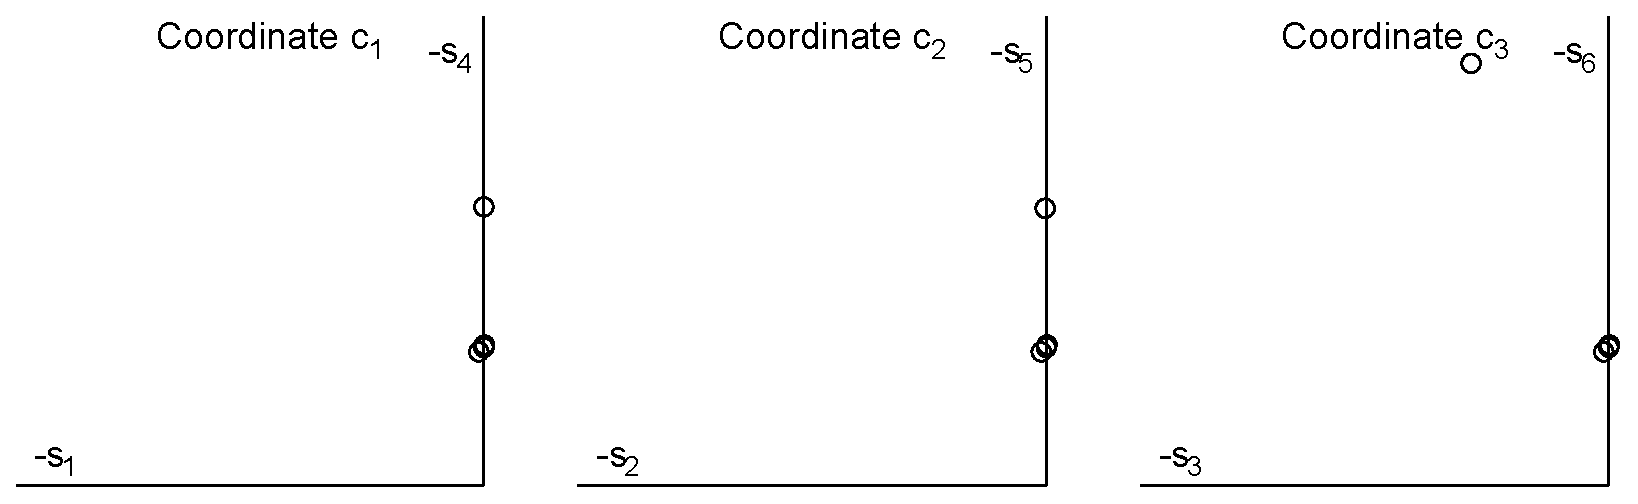
\includegraphics[width=1.0\textwidth]{1_35}
		\caption{Phospholipase A2 unit cells as reported. }
		\label{fig1}
	\end{figure}
	
	\begin{figure}
		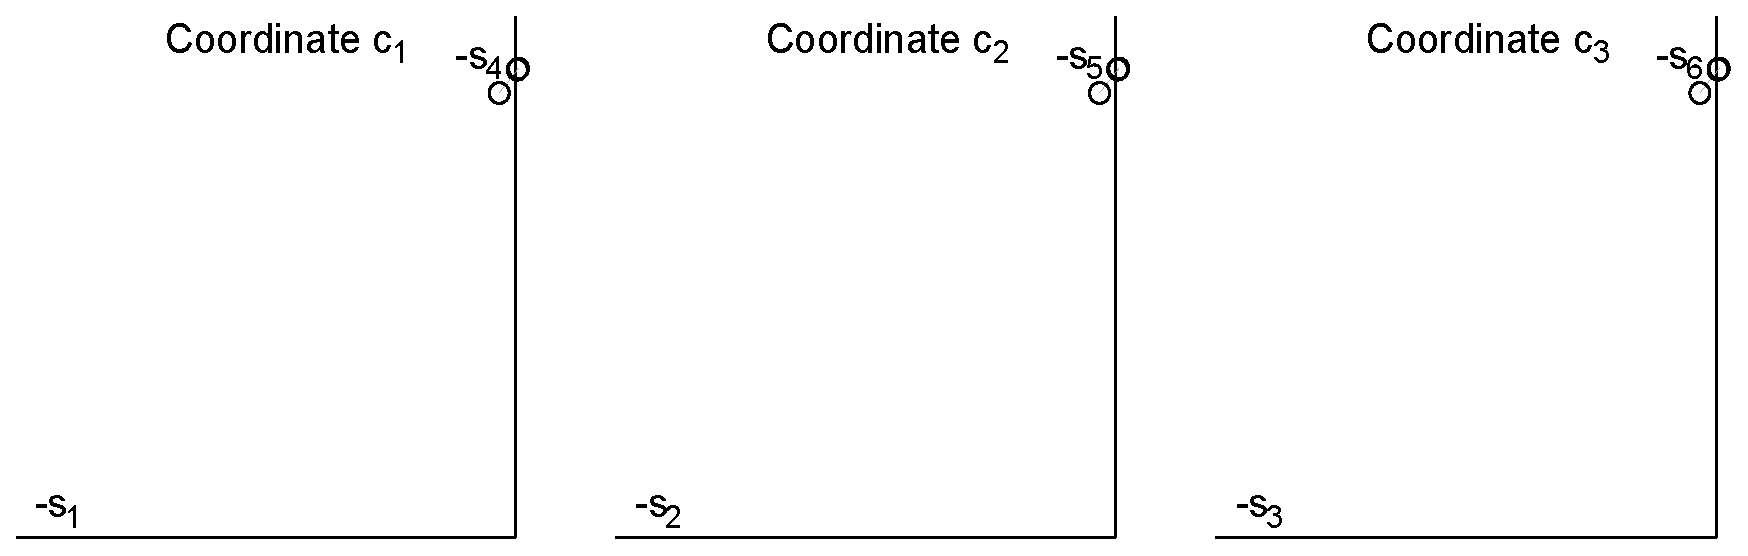
\includegraphics[width=1.0\textwidth]{2_06}
		\caption{The PLA2 unit cells Niggli-reduced. The similarity 
			of the 3 projections is indicative of the exact or nearly
			exact rhombohedral symmetry.}
		\label{fig2}
	\end{figure}
	
\begin{figure}
	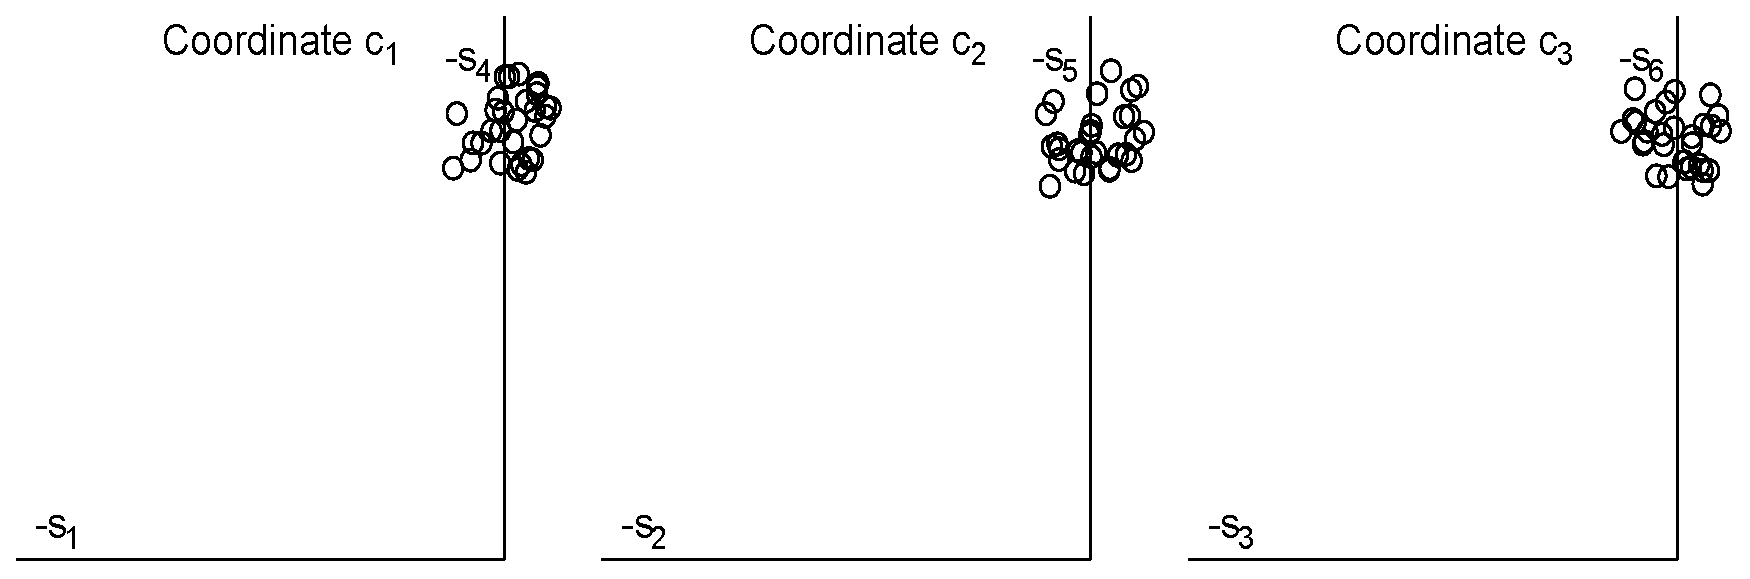
\includegraphics[width=1.0\textwidth]{5_21}
	\caption{The PLA2 unit cells, Niggli-reduced, and five copies were perturbed 10\%
		orthogonally to \SVI{} vector. }
	\label{fig5}	
\end{figure}

\begin{figure}
	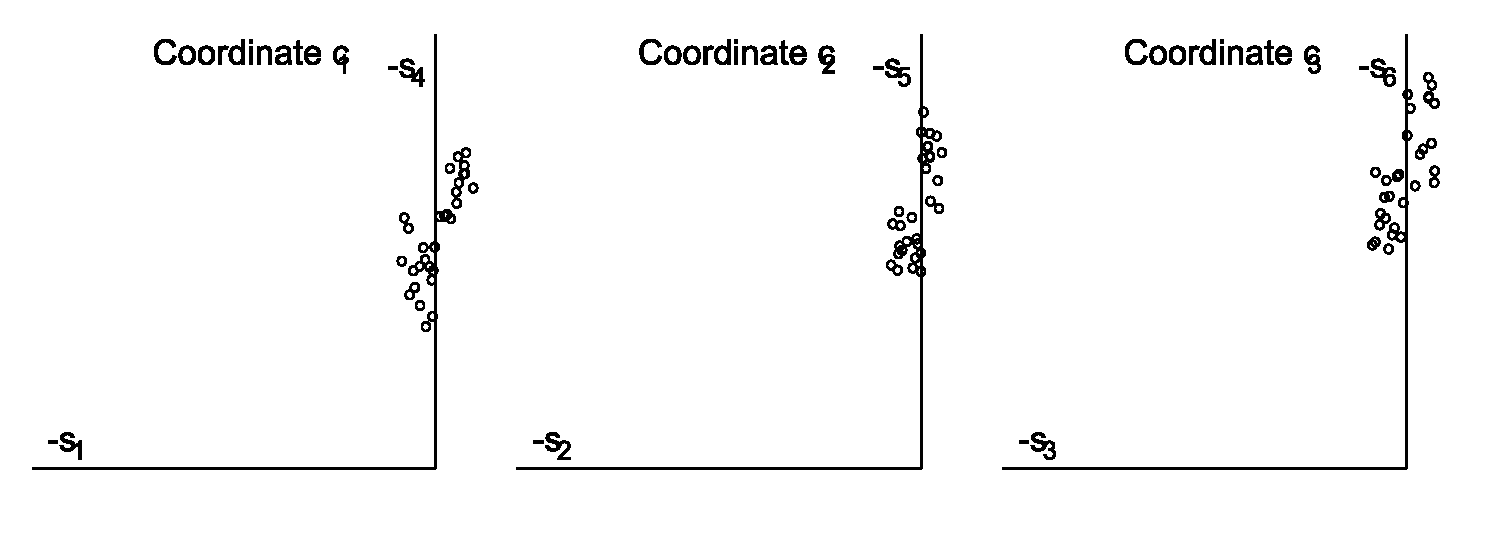
\includegraphics[width=1.0\textwidth]{19_57}
	label{19\_57}
	\caption{The PLA2 unit cells, Niggli-reduced, and five copies were perturbed 10\%
		orthogonally to \SVI{} vector, followed by Niggli reduction.}
\end{figure}

	\begin{figure}
		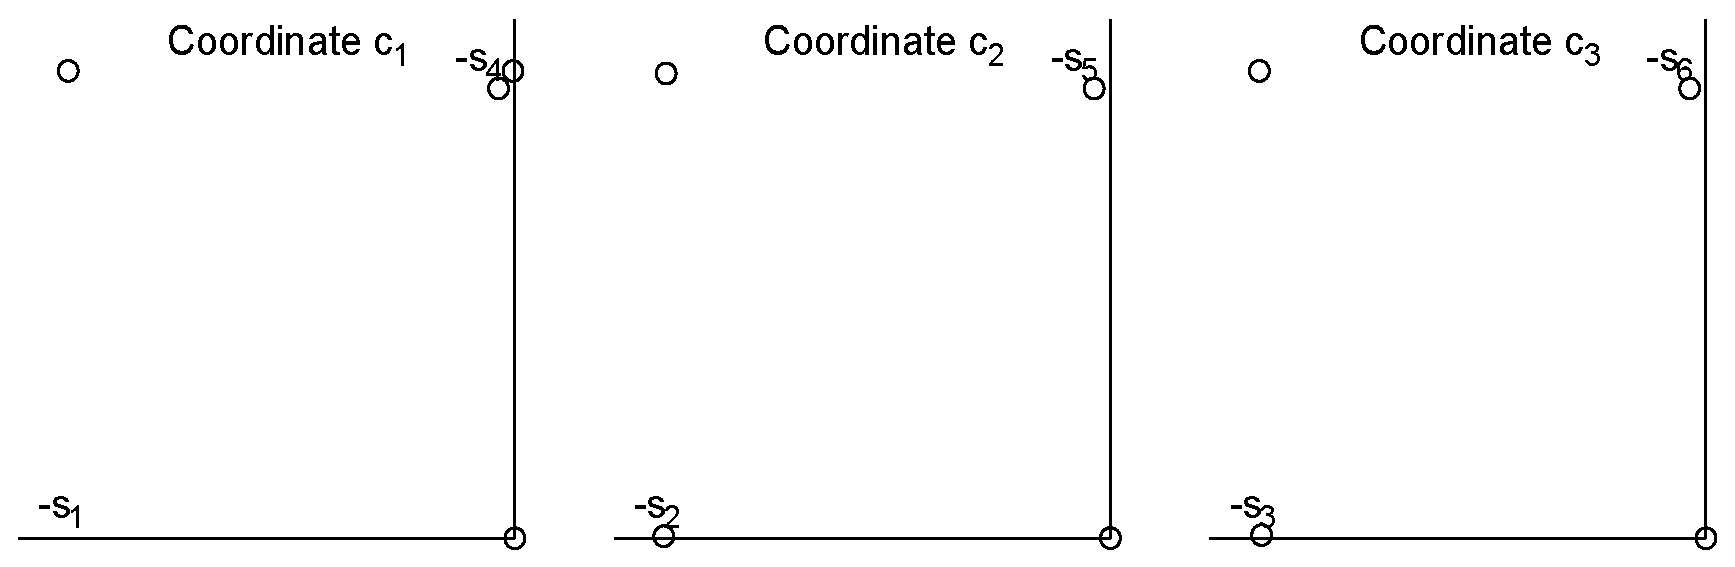
\includegraphics[width=1.0\textwidth]{3_03}
		\caption{The PLA2 unit cells Delone-reduced. }
		\label{fig3}
	\end{figure}
	
	\begin{figure}
		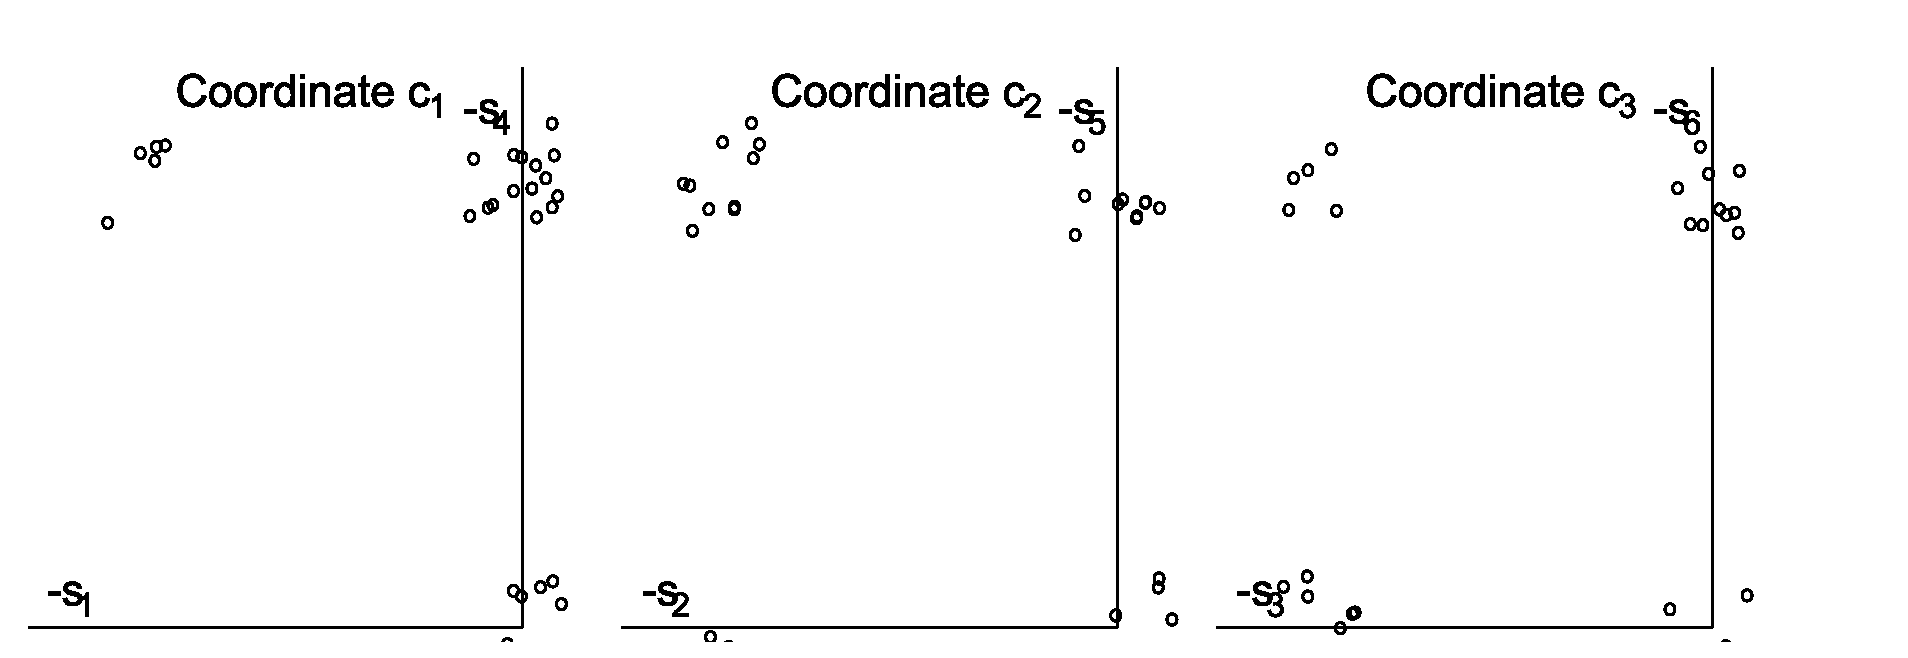
\includegraphics[width=1.0\textwidth]{5_38}
		\label{5_38}
		\caption{The PLA2 cells Delone reduced and
		5 copies perturbed by 10\%.}
	\end{figure}
	
	\begin{figure}
		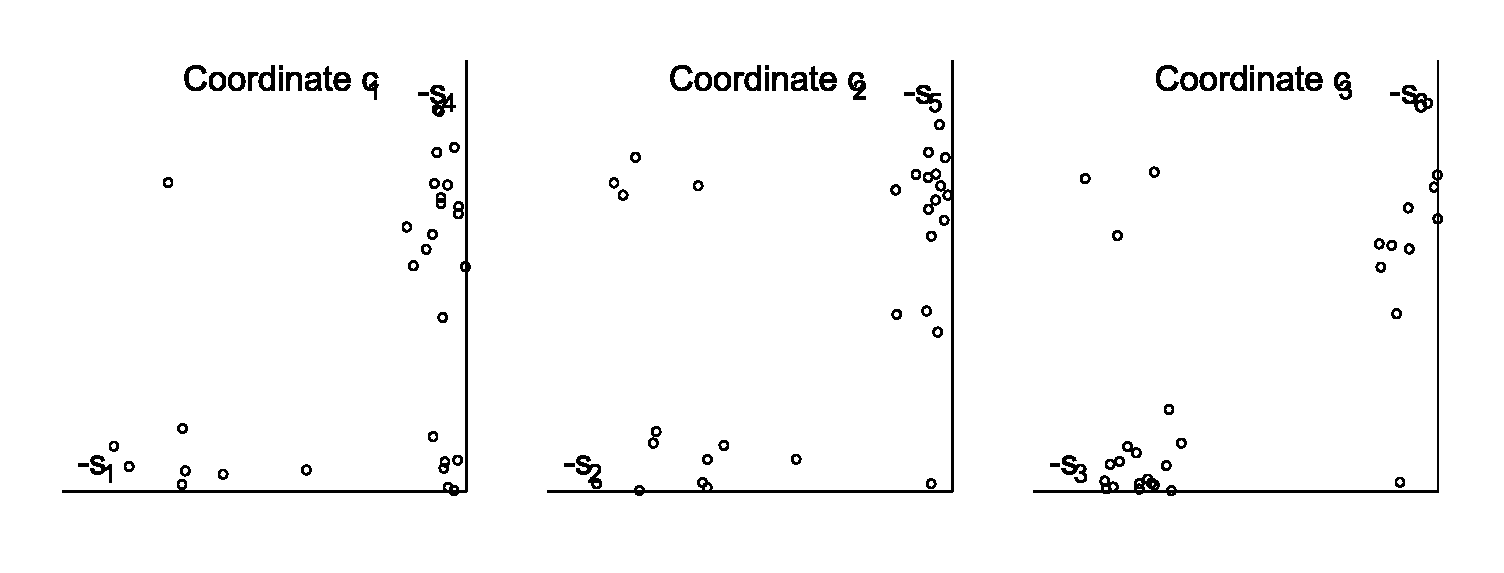
\includegraphics[width=1.0\textwidth]{6_53}
		\label{6_53}
		\caption{The same cells as plotted in Figure \ref{5_38} 
			and Delone reduced.}
	\end{figure}
	
\begin{figure}
	\includegraphics[width=1.0\textwidth]{7_14}
	\label{7_14}
		\caption{The same cells as plotted in Figure \ref{5_38} 
	and Delone reduced, and then each multiplied by the 24
	\SVI{} reflections.}
\end{figure}
	
	\section{Summary}
	
	The transformation matrices shown above demonstrate the 
	considerable regularity of Selling reduction, as used by 
	Delaunay (1932). The reduction operations of Niggli 
	reduction \cite{Niggli1928} are more complex. 
	While all the boundaries of the non-positive 
	orthant of \SVI{} are essentially the same (and 
	related by reflections), the boundaries formed in 
	Niggli reduction are of multiple types, and the fundamental unit 
	of the space representing Niggli-reduced cells (\GVI{}, see \citeasnoun{Andrews2014}) is non-convex.
	
	Several aspects of \CIII{} are evident from inspecting the matrices. 
	First, each boundary has four possible 
	transformations that can be applied. Since each of 
	the transformations at boundaries are self-inverse, they are the 
	same transformations that would be used in the process of 
	cell (lattice) reduction. \citeasnoun{Delaunay1932} and \citeasnoun{Delone1975} give only two choices, presumably for simplicity, 
	omitting transformations that use the ``exchange'' operator 
	(see \citeasnoun{andrews2019b}).
	
	
	
	
	
	
	\section{Availability of code}
	
	The $C^{++}$ ~code for \CIII{} and related 
	software tools is available in github.com, in
	\url{https://github.com/duck10/LatticeRepLib.git}.
	The program CmdToC3 uses the required files.
	
	%\appendix
	
	
	%\section{blah blah blah -- Supplementary Material}
	\ack{{\bf Acknowledgements}}
	
	Careful copy-editing and corrections by Frances C. Bernstein are 
	gratefully acknowledged.
	Our thanks to Jean Jakoncic and Alexei Soares for 
	helpful conversations and access to data and facilities at 
	Brookhaven National Laboratory.
	
	\ack{{\bf Funding information}}      
	
	Funding for this research was provided in part by:  
	US Department of Energy Offices of Biological and 
	Environmental Research and of Basic Energy Sciences 
	(grant No. DE-AC02-98CH10886; grant No. E-SC0012704); 
	U.S. National Institutes of Health (grant No. P41RR012408; 
	grant No. P41GM103473; grant No. P41GM111244; 
	grant No. R01GM117126,
	grant No. 1R21GM129570); Dectris, Ltd.
	
	
	\bibliography{Reduced}
	
	\bibliographystyle{iucr}
	
	
	
	%-------------------------------------------------------------------------
	% TABLES AND FIGURES SHOULD BE INSERTED AFTER THE MAIN BODY OF THE TEXT
	%-------------------------------------------------------------------------
	
	% Simple tables should use the tabular environment according to this
	% model
	
	% Postscript figures can be included with multiple figure blocks
	
	%C:\Users\lca\Source\Repos\LatticeRepLib\x64\Debug>plotc3
	%; Graphical output SVG file =PLT__2023-03-07.13_43_35.svg
	%
	%C:\Users\lca\Source\Repos\LatticeRepLib\x64\Debug>cmdniggli | plotc3
	%; Graphical output SVG file =PLT__2023-03-07.13_44_06.svg
	%
	%C:\Users\lca\Source\Repos\LatticeRepLib\x64\Debug>cmddelone | plotc3
	%; Graphical output SVG file =PLT__2023-03-08.07_11_03.svg
	%
	%C:\Users\lca\Source\Repos\LatticeRepLib\x64\Debug>cmdniggli | cmdperturb 5 20 | plotc3
	%; Graphical output SVG file =PLT__2023-03-08.09_00_13.svg
	%
	%C:\Users\lca\Source\Repos\LatticeRepLib\x64\Debug>cmdniggli | cmdperturb 5 100 | plotc3
	%; Graphical output SVG file =PLT__2023-03-08.09_00_21.svg
	
\end{document}                    % DO NOT DELETE THIS LINE
%%%%%%%%%%%%%%%%%%%%%%%%%%%%%%%%%%%%%%%%%%%%%%%%%%%%%%%%%%%%%%%%%%%%%%%%%%%%%%
